\documentclass[border=.2cm]{standalone}
\usepackage{tikz}
\usepackage{amsmath}
\usetikzlibrary{angles}

\begin{document}

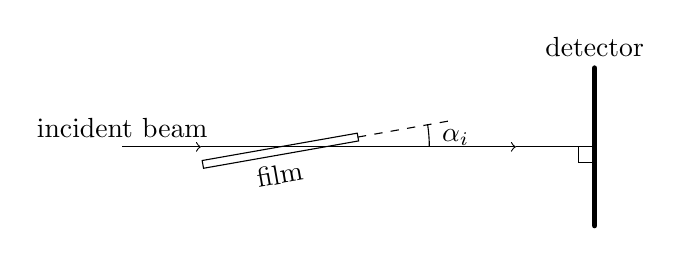
\begin{tikzpicture}
    \draw[rotate=10] (-1, 0) -- (1, 0) --++ (0, -.1) --++ (-2, 0) -- cycle;
    \draw[rotate=10, dashed] (1, -0.05) --++ (1.26, 0) coordinate(tip) node[anchor=north] {$\alpha_i$};
    \draw (0, 0) coordinate(O) --++ (-1,0);
    \draw[<-] (-1, 0) --++ (-1, 0) node[anchor=south] {incident beam};
    \draw[->] (0, 0) --++ (3, 0) coordinate(right);
    \node[rotate=10] at (0, -.35) {film};
    \draw pic [draw, angle radius=1.9cm] {angle = right--O--tip};
    \def\ra{.2};
    \draw (right) --++ (1, 0) ++ (-\ra, 0) --++ (0, -\ra) --++ (\ra, 0);
    \draw[line width=2, cap=round] (right) ++ (1, 1) node[anchor=south] {detector} --++ (0, -2);
\end{tikzpicture}

\end{document}